\section{Tiny Tapeout 3}
\label{sec:tinytapeout3}

Tiny Tapeout 3 opened in March 2023 and 100 new designs were submitted. To fill the remaining space, an additional 149 designs were added from TT01. 
The finished design was submitted for fabrication on Efabless chipIgnite 2304C.
For Tiny Tapeout 3 the two clock buffers of Tiny Tapeout 1 and 2 were replaced by an inverting clock buffer design, with only one buffer between the clock input and output. Fig. ~\ref{fig:TT02_vs_TT03} shows a comparison between the TT02 and TT03 clock buffer designs. By inverting the clock between each design any asymmetry in the clock pulse is evenly spread across the negative and positive cycles.

\begin{figure}[!t]
\centering
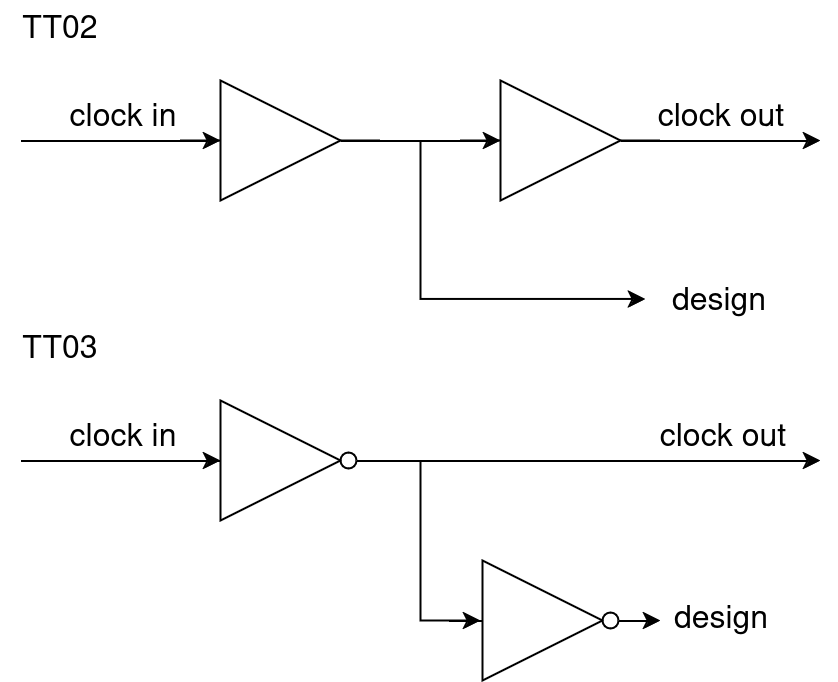
\includegraphics[width=\columnwidth]{./Figs/tt02 vs tt03 scanchain clock.png}
\caption{The Tiny Tapeout 3 architecture buffers the output from the clock network into each design. Clock polarity is alternated between designs to minimize asymmetry between positive and negative cycles.}
\label{fig:TT02_vs_TT03}
\end{figure}

Silicon was received in January 2024, and at the time of writing is being assembled for delivery to customers by March 2024.

Following the closure of Tiny Tapeout 3, an invitational experimental shuttle dubbed Tiny Tapeout 3.5 ~\cite{tinytapeout03p5} was submitted for production. This featured 32 designs, testing and previewing some of the changes planned for Tiny Tapeout 4, detailed in the next section.  Two of these designs included a power gate as a stepping stone to supporting analog and mixed signal designs. 
The finished design was submitted for production on Efabless chipIgnite 2306C.
Silicon was received in December 2023 and at the time of writing is being assembled for testing.

%Again, this needs expansion. Maybe each Tiny Tapeout section should start with a paragraph detailing when it opened for submissions, when it closed, how many submissions there were, when and on what shuttle it was sent for manufacture, and when hardware was received (or when it will be received, where it hasn't arrived yet.
